% -*- TeX -*- -*- UK -*- -*- BMR -*-
% ----------------------------------------------------------------
% Beamer presentation ************************************************
%
% Subhaneil Lahiri's template
%
% To compile:
%   Ctrl-Shift-P
%
% **** -----------------------------------------------------------
\documentclass{beamer}%[hyperref={backref=slide}]
\usetheme{Madrid}

%---------Packages-------------------------------------------------------

\AtBeginSection[]{\frame{\sectionpage}}

% For double screen:
\usepackage{pgfpages}
\setbeameroption{show notes on second screen=right}
%
% For finding documentation:
%\usepackage[centertags]{amsmath}
%\usepackage{amssymb}
%\usepackage{xcolor}
%\usepackage{pgf}
%\usepackage{graphicx}
%\usepackage{hyperref}
%
%\usepackage{ifpdf}
\ifpdf
\else
 \DeclareGraphicsRule{.png}{eps}{.bb}{}
\fi
\usepackage{multimedia}
%\usepackage{epspdfconversion}
\usepackage{epstopdf}
\epstopdfsetup{update,suffix=-generated}
%---------------------------------------
%\usepackage{etoolbox}
%\AtBeginEnvironment{frame}{\pdfbookmark[2]{\noexpand\insertframetitle}{\noexpand\thepage}}

%---Back references---------------------
\usepackage[hyperpageref]{backref}
\renewcommand*{\backref}[1]{}
\renewcommand*{\backrefalt}[4]{%
 \ifcase #1 %
  %
 \or
  #2
 \else
  #2
 \fi
}
\renewcommand*{\backrefentrycount}[2]{\beamerbutton{#1}}
\renewcommand*{\backrefsep}{ }
\renewcommand*{\backreftwosep}{ }
\renewcommand*{\backreflastsep}{ }

%---------Colours---------------------------------------------------------

% \newrgbcolor{LemonChiffon}{1. 0.98 0.8}
% \newrgbcolor{myellow}{.9 .8 .1}
% \newrgbcolor{myblue}{.2 .36 .77}
% \newrgbcolor{orange}{0.8 0.7 0.2}
% \newrgbcolor{myred}{0.95 0.0 0.0}
\definecolor{darkgrey}{rgb}{.5 .5 .5}
\definecolor{darkblue}{rgb}{0.27843137 0.27058824 0.5372549}
\definecolor{darkred}{rgb}{0.5372549 0.27843137 0.27058824}

%---------Commands-------------------------------------------------------

\newcommand{\rref}[1]{\hfill {\small{\color{darkgrey} [#1]}}}
\newcommand{\rrref}[1]{ {\color{darkgrey} #1}}
\newcommand{\citerr}[1]{\hfill {\footnotesize{\color{darkgrey}\cite{#1}}}}

\input{mydefs.tex}
\input{slidesymb.tex}
\input{units.tex}

\newcommand{\hs}{head-sweep}
\newcommand{\Hs}{Head-sweep}


%---------Title-----------------------------------------------------------

\title[Motor programs in Drosophila larvae]{The motor programs underlying navigation in \emph{Drosophila} larva}
%
\subtitle{\small{based on \href{http://dx.doi.org/10.1371/journal.pone.0023180}{\emph{PLoS
  ONE}, 6:\penalty0e23180 (2011)},
  with  K.~Shen, M.~Klein, A.~Tang, E.~Kane, M.~Gershow, P.~Garrity, and A.D.T.~Samuel}\nocite{Lahiri2011}}
%
\author{Subhaneil Lahiri%\inst{1}
}
%
\institute[Harvard]{%
%\inst{1}
Harvard University
}
%
%\slideCaption{}

%---------Beginning--------------------------------------------------------

\begin{document}

%-------------Slide--------------------------------------------------------

\begin{frame}
%
 \titlepage
%
\end{frame}

%-------------Slide--------------------------------------------------------

\begin{frame}{Introduction}
%
 We will look at the motor behaviour of the \emph{Drosophila} larva during navigational motion, paying attention to which segments are used, in which order, etc.
 \note[item]{Ultimately: trace out full pathway sensory $to$ decision $to$ motor}

 \vp We want to get some insight into the circuits that control this behaviour and the role of sensory feedback by quantifying the motor output at high resolution.
 \note[item]{future: interfere, now: just look at normal behaviour}

%
\end{frame}


%-------------Slide--------------------------------------------------------

\begin{frame}{Drosophila larva}
%
 \parbox{5cm}{
   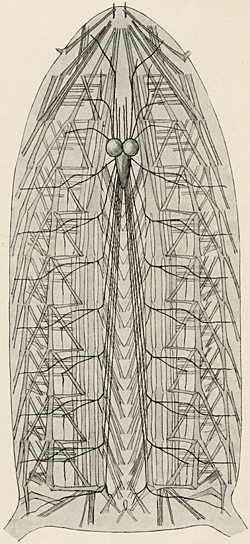
\includegraphics[width=3cm]{Figs/HertweckNervousSys.png}\\
   \rref{Hertweck (1931)}
 }
 \parbox{6cm}{
   $\sim10^4$ neurons.\note[item]{factor of 10 $<$ adult}

   \vp Has CNS, spiking neurons,\ldots\note[item]{unlike c. elegans}

   \vp Many genetic tools.\note[item]{sequenced genome, GAL4/UAS system - target cell types}

   \vp Transparent $\implies$ optogenetics.
 }
%
\end{frame}

%%-------------Slide--------------------------------------------------------
%
%\begin{frame}{Navigation}
%%
% %
% \begin{center}
%   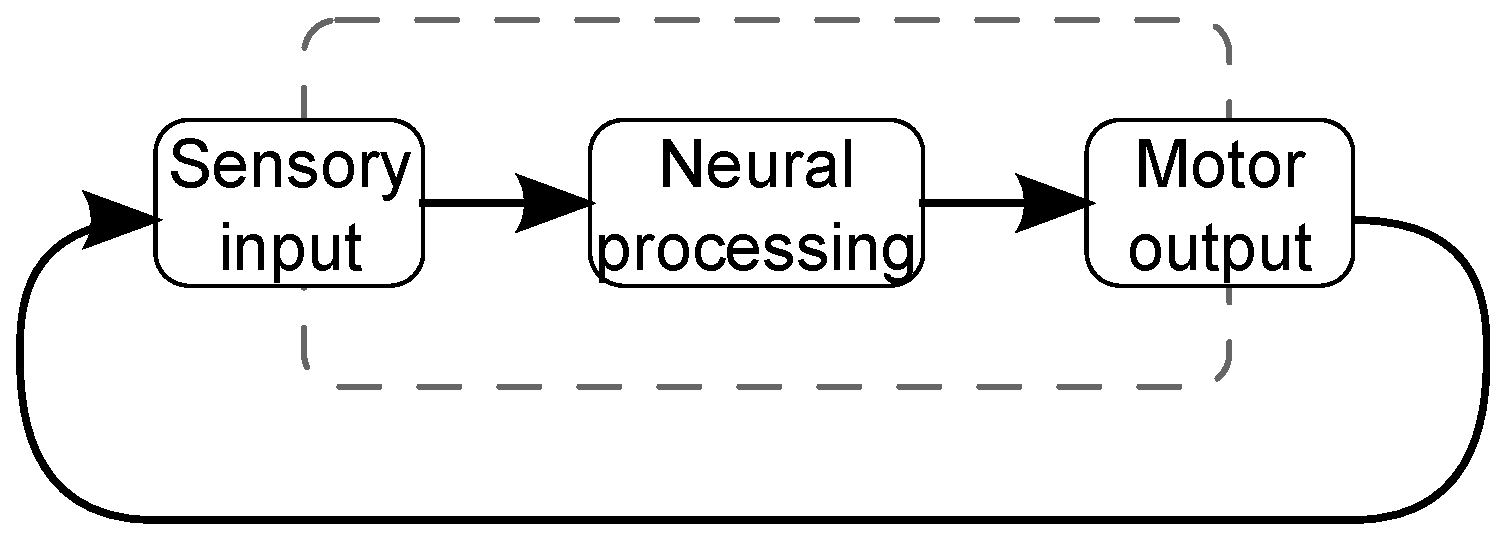
\includegraphics[width=8cm]{Figs/behaviour.eps}
% \end{center}
%
% \vp Relevant sensory inputs can be controlled  easily.\note[item]{Temperature, odour, light}
%
% \vp Large scale motor output can be measured easily. \note[item]{path travelled, turning decisions}
% %
%%
%\end{frame}
%
%-------------Slide--------------------------------------------------------

\begin{frame}{Outline}
%
 \tableofcontents[hideallsubsections]
 \note[item]{review how D.larvae navigate, what's known about locomotion circuits}
 \note[item]{how larvae with fluorescent muscles will help us, how we use them}
 \note[item]{results of this analysis}
 \note[item]{conclusions and future directions}
%
\end{frame}

%-------------Section--------------------------------------------------------

\section{Navigation and locomotion}


%-------------Slide--------------------------------------------------------

\begin{frame}{Biased random walks}
%
 %
 \parbox{5cm}{   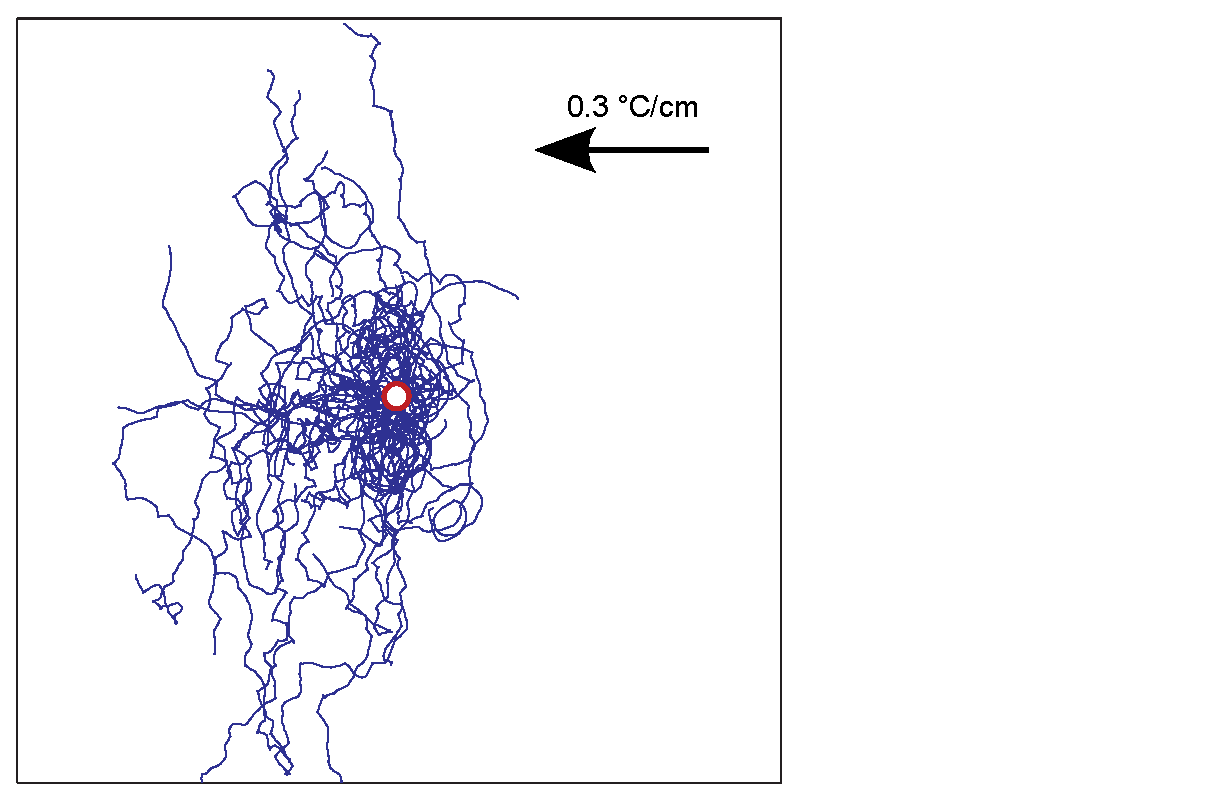
\includegraphics[width=7cm]{Figs/CSandMHCGFPcenteredtracks2.eps} }
 \parbox{6cm}{Alternating runs and reorientations.\note[item]{longer runs in good directions}

 \vp Effectively point-like sensor.\note[item]{has to move sensor to measure gradients}

 \vp Similar to  \emph{E.\ coli} and \emph{C.\ elegans}.\note[item]{can do more}}

 \note[item]{the thing that allows D.larvae to do more...}
%
\end{frame}

%-------------Slide--------------------------------------------------------

\begin{frame}{\Hs s}
%
 \begin{center}
 \movie[width=131px,height=98px,showcontrols=true,loop]
 {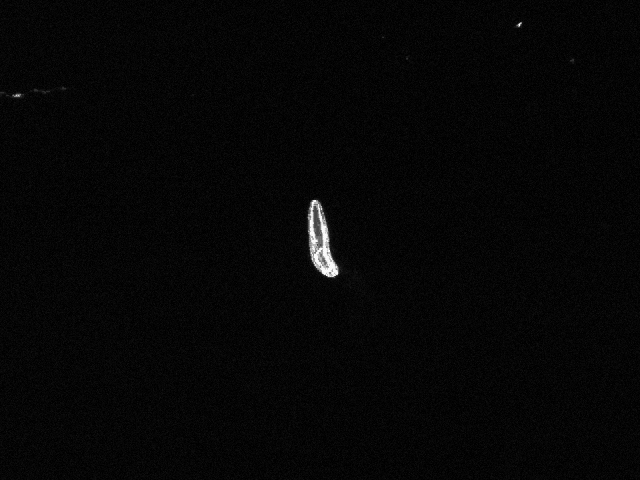
\includegraphics[width=131px,height=98px]{Firstframe/hsa.png}}
 {Vids/hsa.avi}\note[item]{accepted}
 \movie[width=131px,height=98px,showcontrols=true,loop]
 {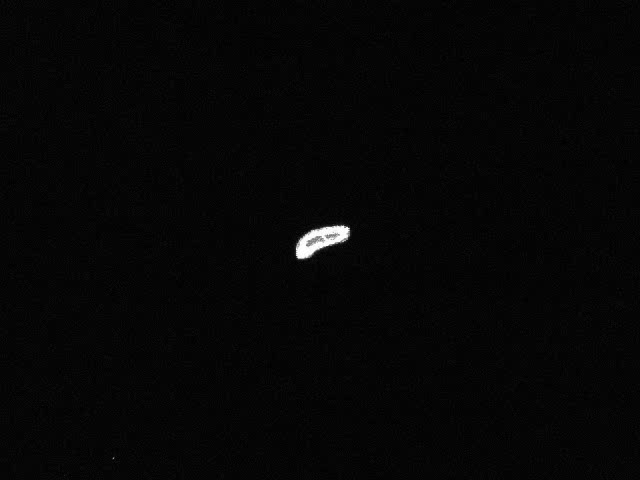
\includegraphics[width=131px,height=98px]{Firstframe/hsr.png}}
 {Vids/hsr.avi}\note[item]{rejected}
 \end{center}
 Moves head from side-to-side to sample environment and pick a direction to travel.
%
\end{frame}

%-------------Slide--------------------------------------------------------

\begin{frame}{Navigation strategy}
%
 For thermo-/chemo-/photo-taxis, larva modulates:
 \begin{itemize}
   \item \hs\ frequency \note[item]{turns more when things are getting worse}
   \item \hs\ size  \note[item]{larger turns when things are getting worse}
   \item \hs\ acceptance probability \note[item]{more likely to accept when better}
 \end{itemize}
 Depending on whether conditions are improving/worsening.

 \citerr{Luo20335462}
%
\end{frame}

%-------------Slide--------------------------------------------------------

\begin{frame}{Questions}
%
 Different types of \hs:
 \begin{itemize}
    \item Different circuits?
    \item When is decision made? With what info?
    \item Mechano-sensory feedback?
  \end{itemize}

  \vp Look for differences in mechanics of different types of \hs.
  \note[item]{difference in initiation $\to$ makes decision before}
%
\end{frame}

%-------------Slide--------------------------------------------------------

\begin{frame}{Locomotion and sensory feedback}\label{fr_loco}%[label=fr_loco]
%
 Crawl using peristaltic waves from posterior to anterior that lift and push the body forwards.
 \note[item]{We'll see lots of videos of this later.}

 \vp Several types of Multidendritic (md) sensory neurons.%:
% \begin{itemize}
%  \item tracheal dendrite (td),
%  \item bipolar dendrite (bd)
%  \item class I-IV dendritic arborisation (da).
% \end{itemize}

 Repeated in each segment.
 Possibly used for proprioception. \\ \citerr{Bodmer1987s,Grueber12050135}

 \vp md neurons are used for locomotion:
 \begin{itemize}
   \item Turn off all types $\to$ no locomotion \citerr{Song17360325}
   \item Turn off %bd and class I da
   certain subsets
   $\to$ disrupt pattern \hyperlink{fr_toothpaste<1>}{(toothpasting)}\\ \citerr{Hughes17498969}%,\citerr{Cheng20696376}
 \end{itemize}
 \note[item]{each segments waits for posterior segment to contract.}

 %\vp For finer analysis: quantify patterns of muscle use.
 \note[item]{in future: interfere}
%
\end{frame}

%-------------Section--------------------------------------------------------

\section{Imaging and analysis of fluorescent muscles}

%-------------Slide--------------------------------------------------------

\begin{frame}{Fluorescent muscles}
%
 \begin{center}
 Mutant: $w^-; \frac{mhc-GFP^{0110}}{CyO}$ \citerr{Hughes17498969}

 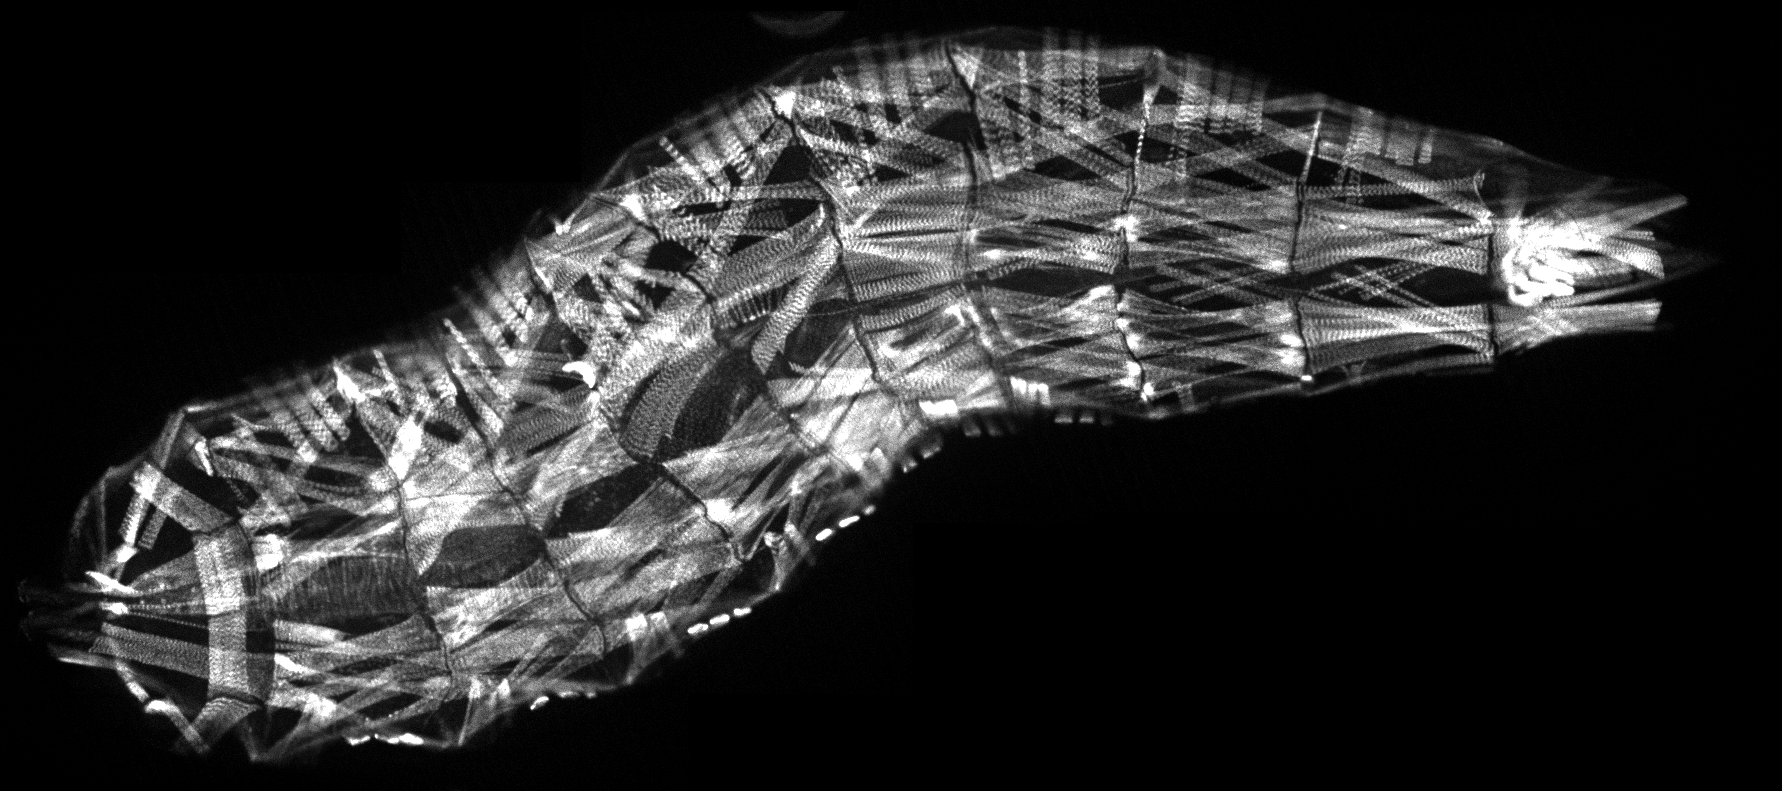
\includegraphics[width=12cm]{Figs/LarvaStitchScaled.png}
 \end{center}
 \note[item]{we see 11 segments, some people talk about A9 (terminal, too small), mouth segment (involute during early development)}

 \vp Can see segment boundaries $\to$ measure length $\to$ which segment contracts.
 \note[item]{can't automate this yet.}
%
\end{frame}

%-------------Slide--------------------------------------------------------

\begin{frame}{Intensity pattern}
%
 \begin{center}
 % divide width/height by 8.
 \movie[width=162px,height=162px,showcontrols=true,loop]
 {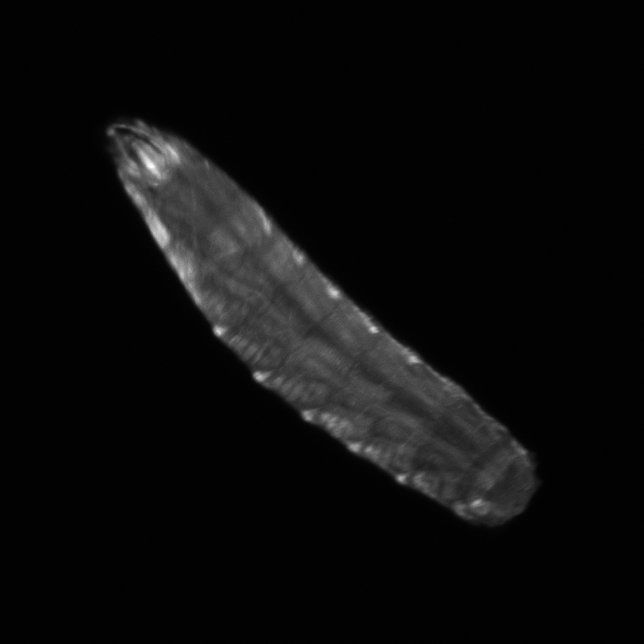
\includegraphics[width=162px,height=162px]{Firstframe/Peristalsis_scaled.png}}
 {Vids/Peristalsis_scaled.avi}
 \end{center}

 Muscles contract $\rightarrow$ same GFP in smaller volume $\rightarrow$ increase
 concentration $\rightarrow$ increase brightness.\note[item]{another measure of contraction. less noisy}

%
\end{frame}

%%-------------Slide--------------------------------------------------------
%
%\begin{frame}{Thermotaxis: mutant vs.\ wild type}
%%
% Varying temperature from $19-21\dC$ with period $5\mins$.
%
% \begin{center}
% Turning rate ($\mathrm{min}^{-1}$)
%
% %\vp
% \begin{tabular}{|r|c|c|}
%   \hline
%   % after \\: \hline or \cline{col1-col2} \cline{col3-col4} ...
%    & wild-type & mhc-GFP \\
%    \hline
%   warming & $2.89 \pm 0.16$ & $2.63 \pm 0.15$ \\
%   cooling & $5.88 \pm 0.21$ & $3.74 \pm 0.14$ \\
%   \hline
% \end{tabular}
%
% \vp Speed ($\mathrm{mm}/\mathrm{s}$)
%
% %\vp
% \begin{tabular}{|c|c|}
%   \hline
%   % after \\: \hline or \cline{col1-col2} \cline{col3-col4} ...
%   wild-type & mhc-GFP \\
%   \hline
%   $0.261 \pm 0.006$ & $0.285 \pm 0.006$ \\
%   \hline
% \end{tabular}
% \end{center}
%%
%\end{frame}
%
%-------------Section--------------------------------------------------------



%-------------Slide--------------------------------------------------------

\begin{frame}{Apparatus}
%
 \parbox{6cm}{
  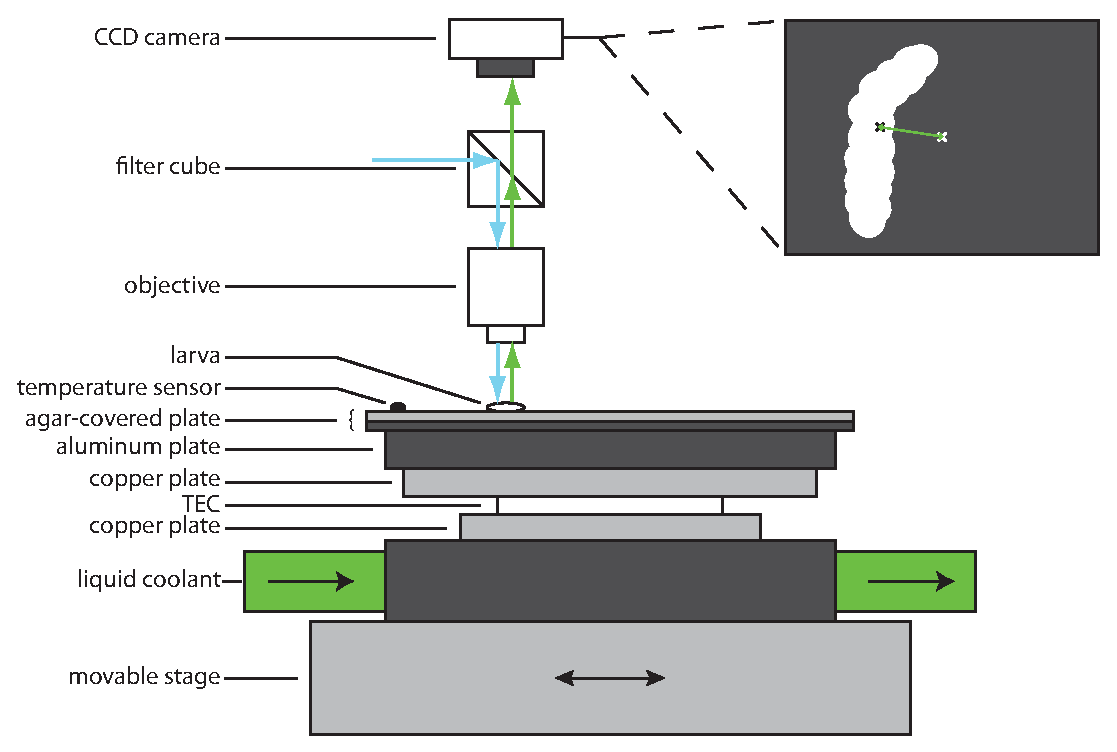
\includegraphics[height=4cm]{Figs/LocomotionApparatus.eps}
 }
 \parbox{5cm}{
  \begin{itemize}
    \item Temperature varied from $14-16\dC$ with period $300\s$.
    \note[item]{triggers many \hs s}
    \note[item]{allows comparison of \hs in warming/cooling}
    \item Movable stage keeps larva in camera frame.
  \end{itemize}
 }
%
\end{frame}

%-------------Slide--------------------------------------------------------

\begin{frame}{Image analysis}
%
 \begin{center}
 \parbox{3cm}{
%  \only<1>{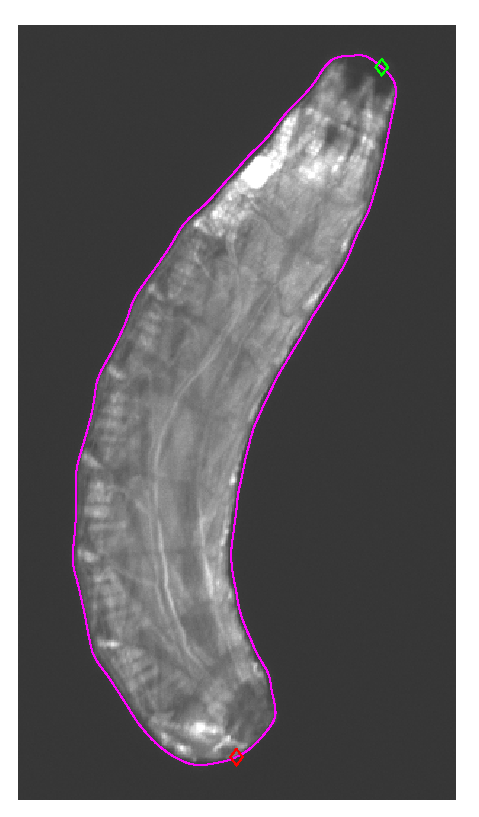
\includegraphics[height=4cm]{Figs/headtail.eps}}
  \only<1>{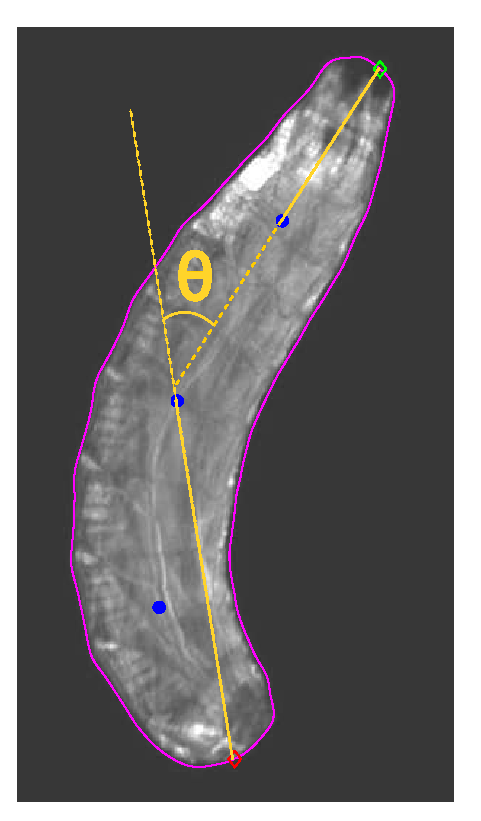
\includegraphics[height=4cm]{Figs/cln.eps}}
  \only<2>{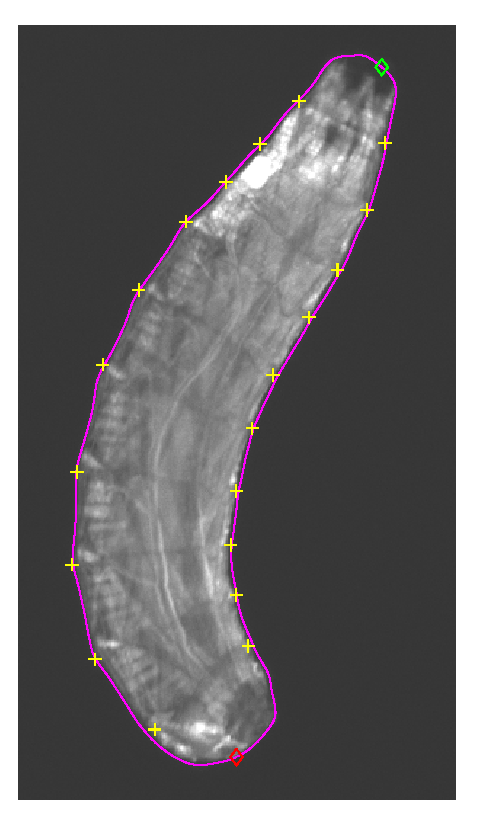
\includegraphics[height=4cm]{Figs/nodes.eps}}
  \only<3>{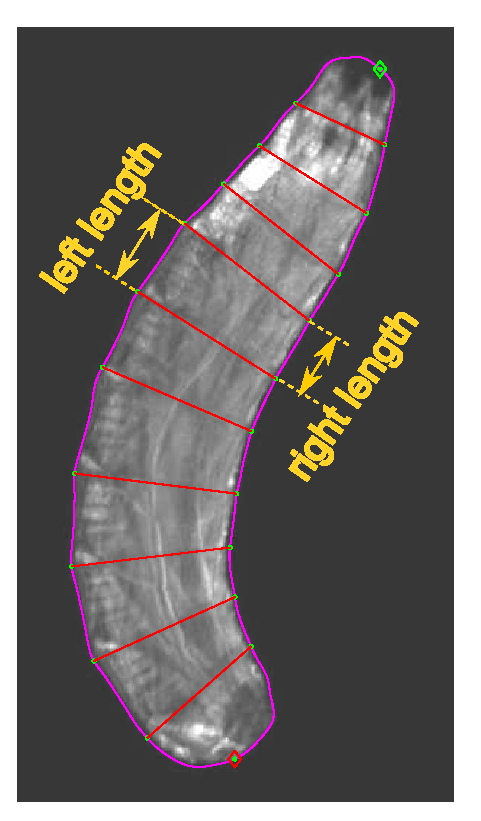
\includegraphics[height=4cm]{Figs/segs.eps}}
  \only<4>{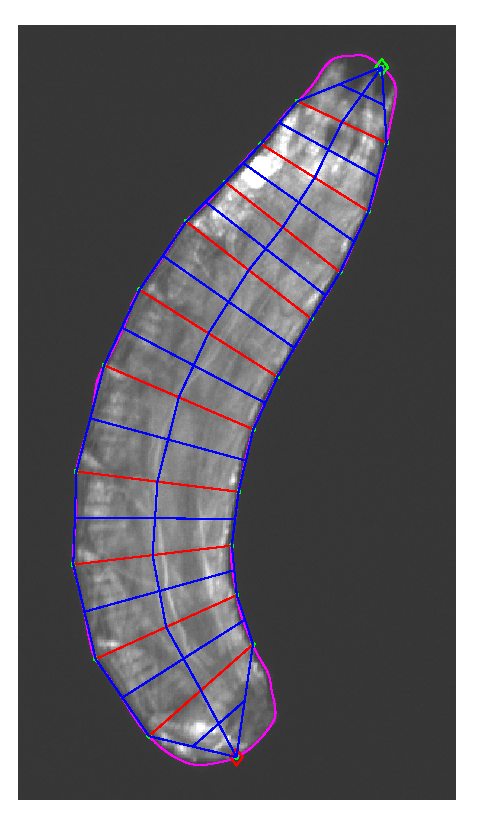
\includegraphics[height=4cm]{Figs/quads.eps}}}
 \end{center}

 \vp
% \only<1>{Find boundary, head and tail automatically}
 \only<1>{Find boundary, head, tail and bend angle automatically}\note[item]{allows us to flag interesting bits}
 \only<2>{User clicks on segment boundaries}\note[item]{slowest part}
 \only<3>{Map to boundary. Find segment lengths.}\note[item]{automatic again. look for asymmetry}
 \only<4>{Split segment into quadrants. Mean pixel value $\to$ intensity.}\note[item]{less noisy}
%
\end{frame}

%%-------------Slide--------------------------------------------------------
%
%\begin{frame}{Intensity vs.\ length}
%%
% \begin{center}
%   \includegraphics[width=5cm]{IntLen/IntLenSegments.eps}
%   \hspace{1cm}
%   \includegraphics[width=5cm]{IntLen/IntLenAnimals.eps}
% \end{center}
%%
%\end{frame}
%
%-------------Slide--------------------------------------------------------

\begin{frame}{Coordinate system}
%
 \note{this slide just to explain how to read graphs. Interpret later.\par}
 \note{\vp thorax -3 to 3, rest abdomen}
 \parbox{5cm}{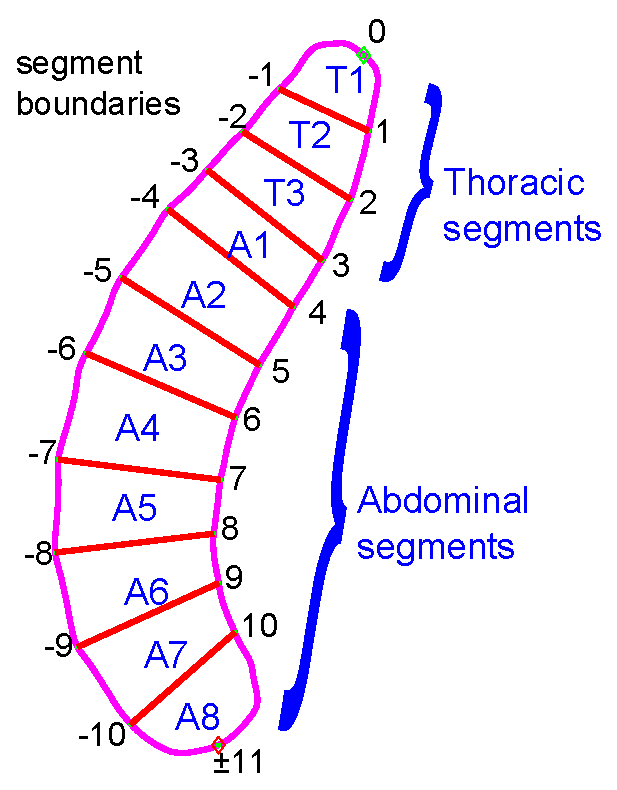
\includegraphics[height=5cm]{Figs/coords.eps}}
 \parbox{5cm}{\only<1>{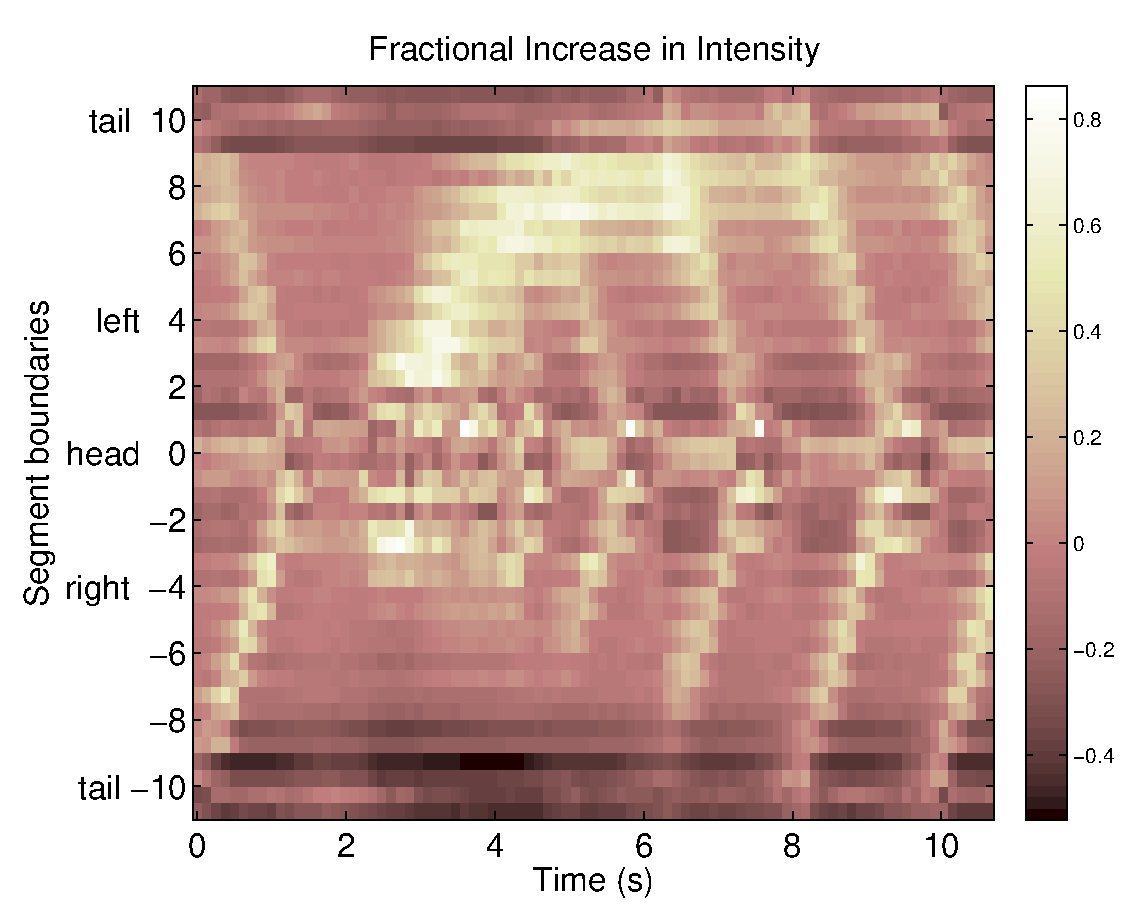
\includegraphics[height=5cm]
                        {Figs/warm_large_left_IntContrIm.eps}}
 \note[item]{Head in middle, left above, right below. \par
 Bright spots: contraction. See peristalsis go from tail to head}
              \only<2>{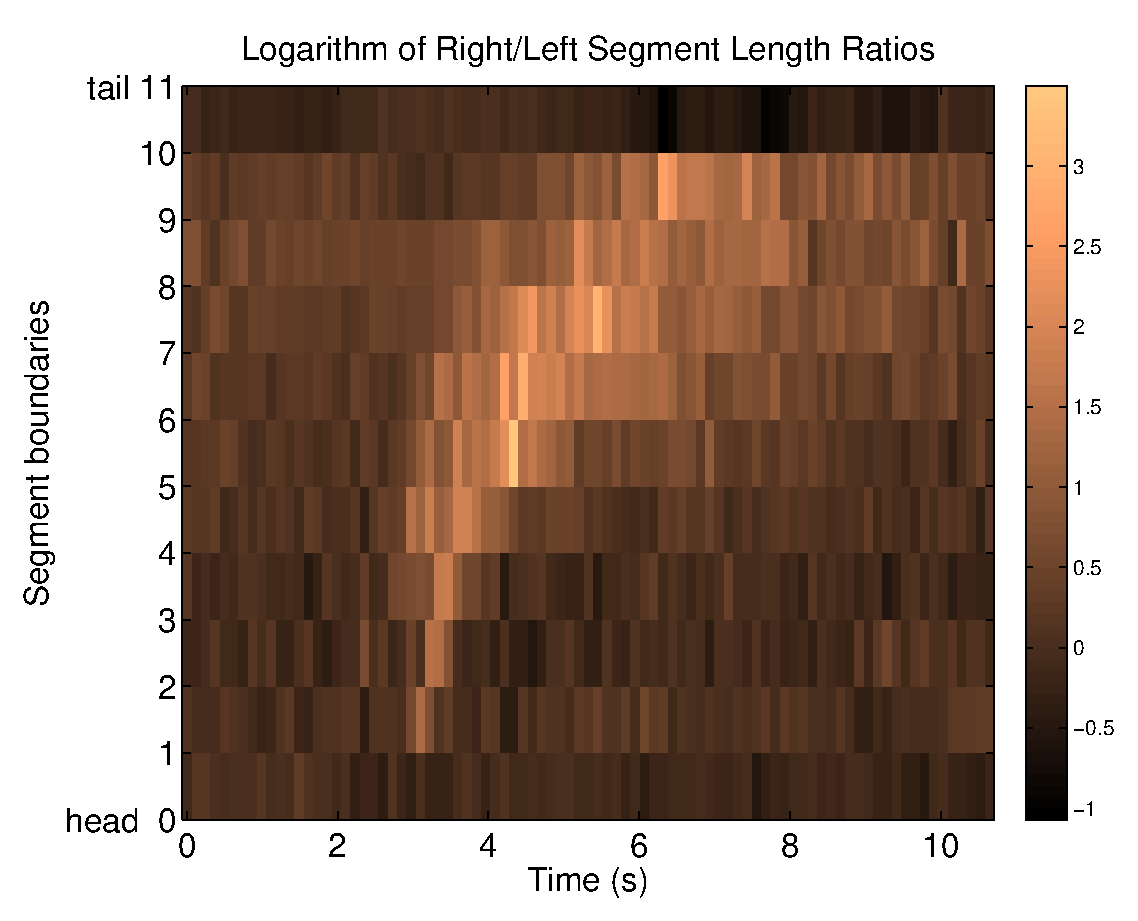
\includegraphics[height=5cm]
                        {Figs/warm_large_left_LenRatioIm.eps}}}
 \note[item]{Head at bottom, tail at top. Remove peristalsis, just see bend.\par
 Bright: left bend, dark: right bend.}

%
\end{frame}

%-------------Section--------------------------------------------------------

\section{Results}

%-------------Slide--------------------------------------------------------

\begin{frame}{Forward motion}
%
 \begin{center}
   \movie[width=315px,height=188px,showcontrols=true,loop]
   {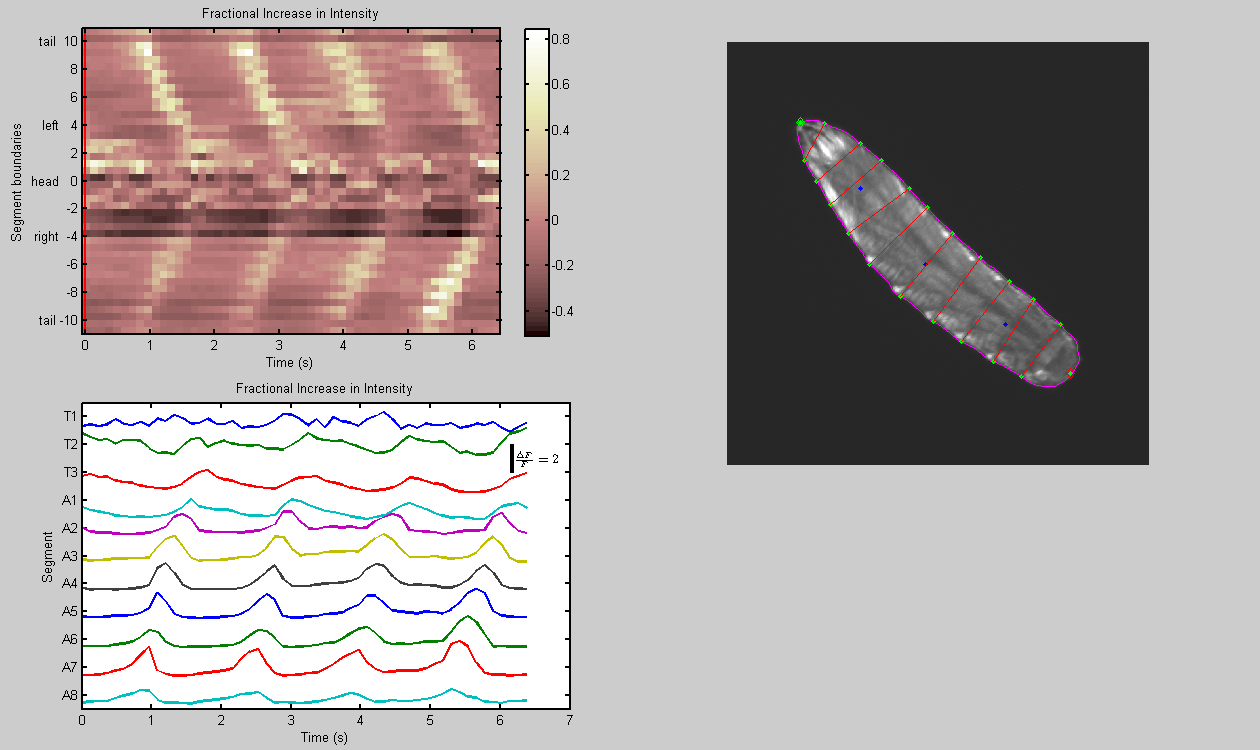
\includegraphics[width=315px,height=188px]{Firstframe/Peristalsis_video.png}}
   {Vids/Peristalsis_video.avi}
 \end{center}
 Pulse travels from tail to head.
 New pulse starts after previous reaches head.
 \note[item]{Mouth hooks drown out all else (ratio) in T1,T2.}
 \note[item]{If we interfere with sensory feedback, could use this to measure effects.}
%
\end{frame}

%-------------Slide--------------------------------------------------------

\begin{frame}{Small accepted \hs}
%
 \begin{center}
   \movie[width=315px,height=188px,showcontrols=true,loop]
   {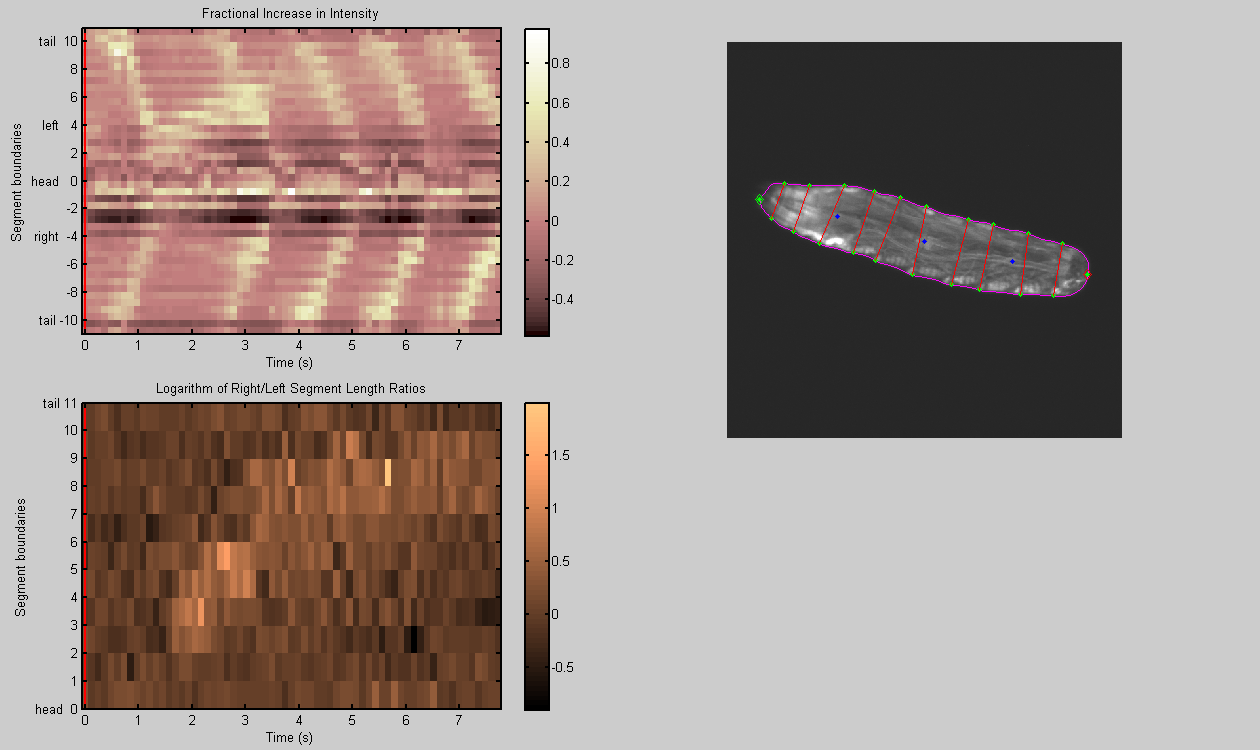
\includegraphics[width=315px,height=188px]{Firstframe/warm_small_left_video.png}}
   {Vids/warm_small_left_video.avi}
 \end{center}

 Basic pattern: Kink starts around (T3,A1,A2) and propagates back.
 Subsequent peristalsis starts before kink reaches tail.
 \note[item]{Completes \hs\ with peristalsis, not unbending.}
 \note[item]{non-overlapping}
%
\end{frame}

%-------------Slide--------------------------------------------------------

\begin{frame}{Large accepted \hs}
%
 \begin{center}
   \movie[width=315px,height=188px,showcontrols=true,loop]
   {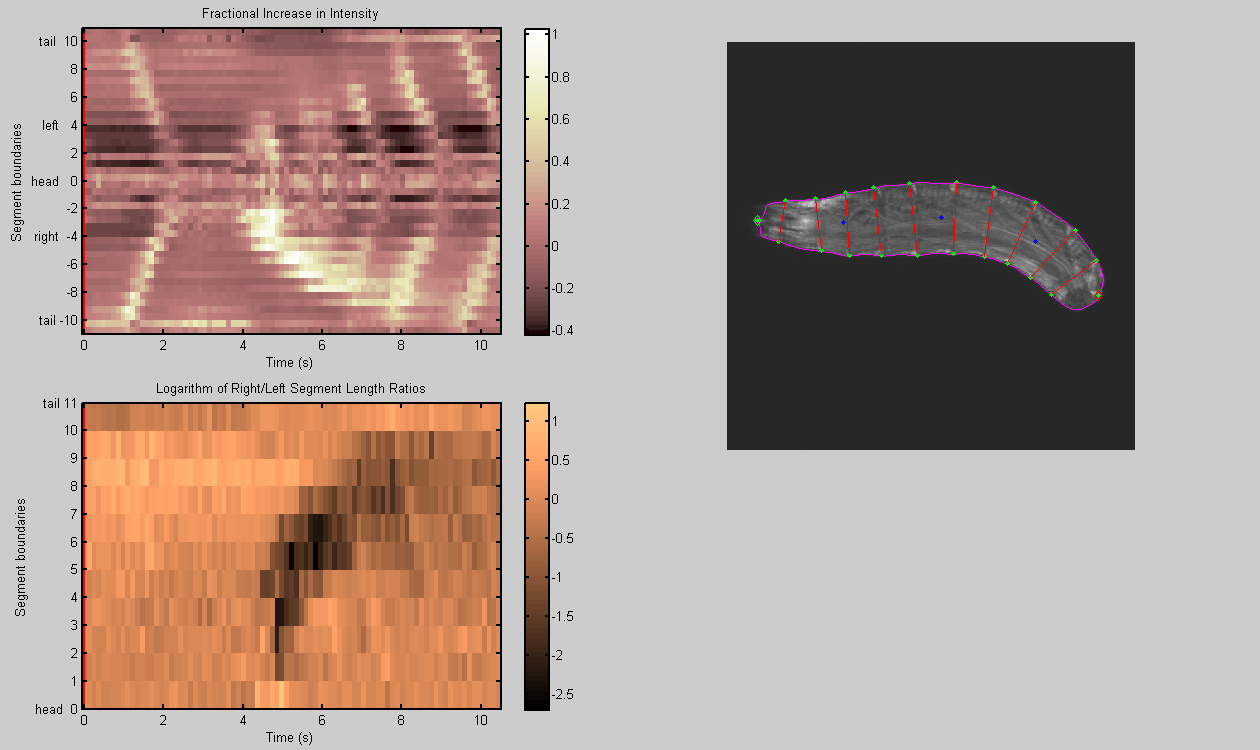
\includegraphics[width=315px,height=188px]{Firstframe/cool_large_right_video.png}}
   {Vids/cool_large_right_video.avi}
 \end{center}

 Basic pattern: Kink starts around (T3,A1,A2) and propagates back.\note[item]{same as small, statistics later}
 Subsequent peristalsis starts from kink, \alert{not} tail.
%
\end{frame}

%-------------Slide--------------------------------------------------------

\begin{frame}{Rejected \hs}
%
 \begin{center}
   \movie[width=315px,height=188px,showcontrols=true,loop]
   {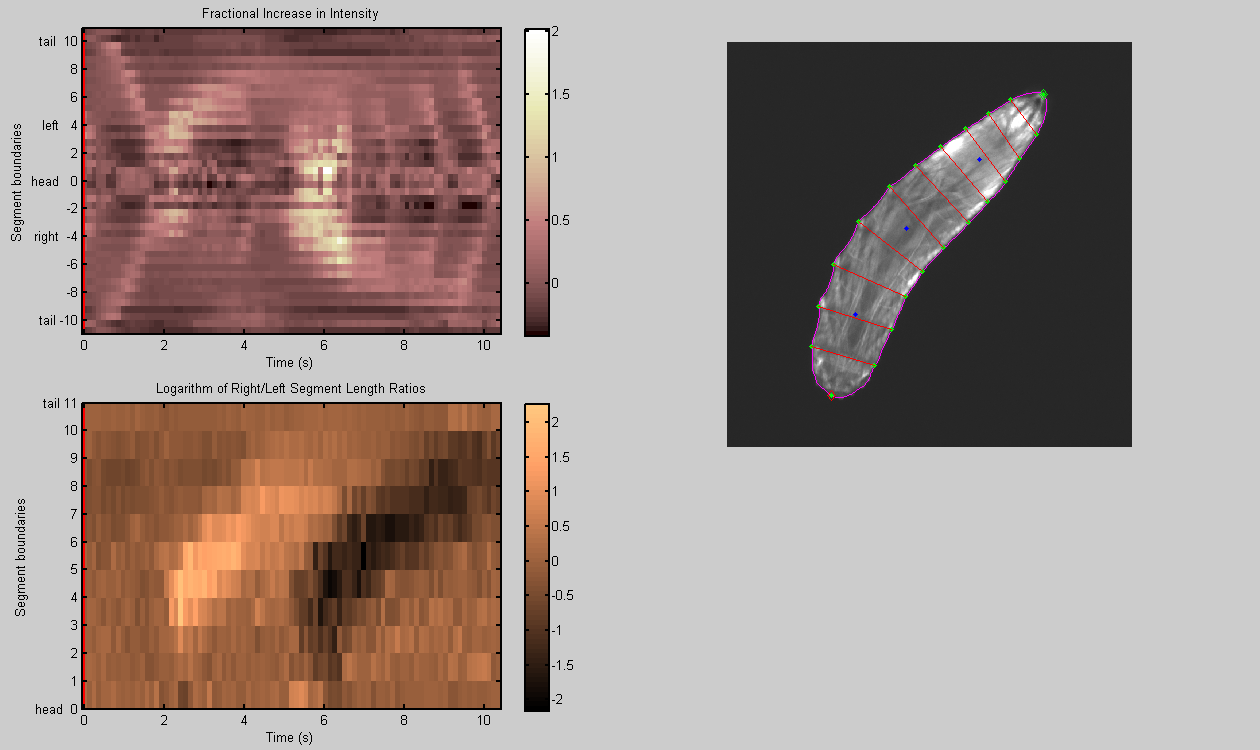
\includegraphics[width=315px,height=188px]{Firstframe/rejected_video.png}}
   {Vids/rejected_video.avi}
 \end{center}
 Rejected \hs\ not undone until next one.\note[item]{no unbending program}
%
\end{frame}

%%-------------Slide--------------------------------------------------------
%
%\begin{frame}{Right vs.\ left turns}
%%
% \begin{center}
%  \parbox{5cm}{\begin{center}Right\end{center}}
%  \hspace{1cm}
%  \parbox{5cm}{\begin{center}Left\end{center}}
%  \only<2>{
%   \includegraphics[width=5cm]{FiguresForPaper/WarmSmallRight/warm_small_right_IntContrIm.eps}
%   \hspace{1cm}
%   \includegraphics[width=5cm]{FiguresForPaper/WarmSmallLeft/warm_small_left_IntContrIm.eps}}
%  \only<1>{
%   \includegraphics[width=5cm]{FiguresForPaper/WarmSmallRight/warm_small_right_LenRatioIm.eps}
%   \hspace{1cm}
%   \includegraphics[width=5cm]{FiguresForPaper/WarmSmallLeft/warm_small_left_LenRatioIm.eps}}
% \end{center}
%
% \vp Same overall pattern.
%%
%\end{frame}
%
%%-------------Slide--------------------------------------------------------
%
%\begin{frame}{Warming vs.\ cooling}
%%
% \begin{center}
%  \parbox{5cm}{\begin{center}Warming\end{center}}
%  \hspace{1cm}
%  \parbox{5cm}{\begin{center}Cooling\end{center}}
%  \only<2>{
%   \includegraphics[width=5cm]{FiguresForPaper/WarmSmallLeft/warm_small_left_IntContrIm.eps}
%   \hspace{1cm}
%   \includegraphics[width=5cm]{FiguresForPaper/CoolSmallLeft/cool_small_left_IntContrIm.eps}}
%  \only<1>{
%   \includegraphics[width=5cm]{FiguresForPaper/WarmSmallLeft/warm_small_left_LenRatioIm.eps}
%   \hspace{1cm}
%   \includegraphics[width=5cm]{FiguresForPaper/CoolSmallLeft/cool_small_left_LenRatioIm.eps}}
% \end{center}
%
% \vp No difference in pattern.
%%
%\end{frame}
%
%%-------------Slide--------------------------------------------------------
%
%\begin{frame}{Small vs.\ large angles}
%%
% \begin{center}
%  \parbox{5cm}{\begin{center}Small ($48^\circ$) \end{center}}
%  \hspace{1cm}
%  \parbox{5cm}{\begin{center}Large ($108^\circ$) \end{center}}
%  \only<2>{
%   \includegraphics[width=5cm]{FiguresForPaper/WarmSmallRight/warm_small_right_IntContrIm.eps}
%   \hspace{1cm}
%   \includegraphics[width=5cm]{FiguresForPaper/CoolLargeRight/cool_large_right_IntContrIm.eps}}
%  \only<1>{
%   \includegraphics[width=5cm]{FiguresForPaper/WarmSmallRight/warm_small_right_LenRatioIm.eps}
%   \hspace{1cm}
%   \includegraphics[width=5cm]{FiguresForPaper/CoolLargeRight/cool_large_right_LenRatioIm.eps}}
% \end{center}
%
% \vp Same basic pattern for turn.
% \visible<2>{Small: subsequent peristalsis starts from tail. Large: starts from kink.}
%%
%\end{frame}
%
%%-------------Slide--------------------------------------------------------
%
%\begin{frame}{Large \Hs}
%%
% \begin{center}
%   \movie[width=315px,height=188px,showcontrols=true,loop,poster]{}
%   {FiguresForPaper/CoolLargeRight/cool_large_right_video.avi}
% \end{center}
%%
%\end{frame}
%
%-------------Slide--------------------------------------------------------

\begin{frame}{Position of initial bend}
%
 \begin{center}
   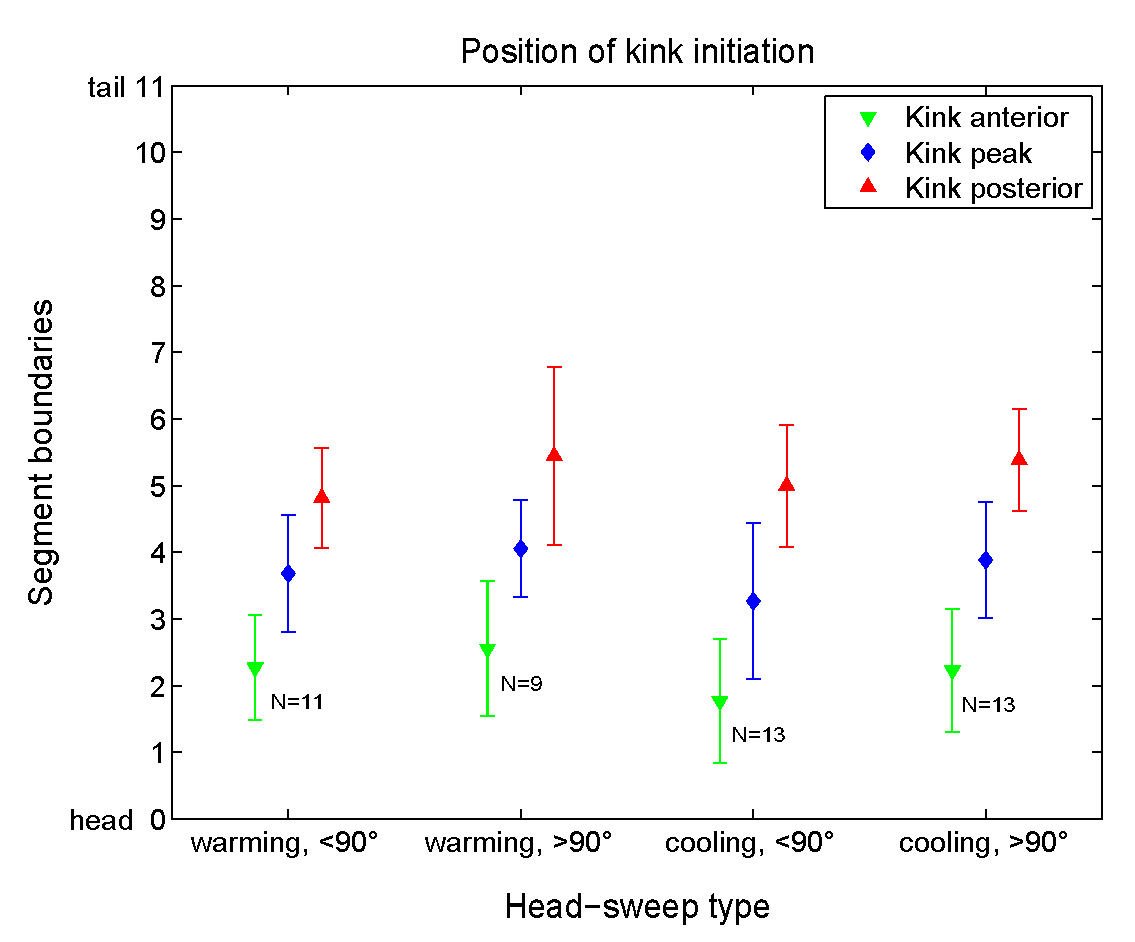
\includegraphics[height=6cm]{Figs/KinkStart.eps}
 \end{center}
 \note[item]{error bars ar std dev, not std err.}

 Little dependence on size or temperature.
%
\end{frame}

%-------------Slide--------------------------------------------------------

\begin{frame}{Position of start of peristalsis}
%
 \begin{center}
   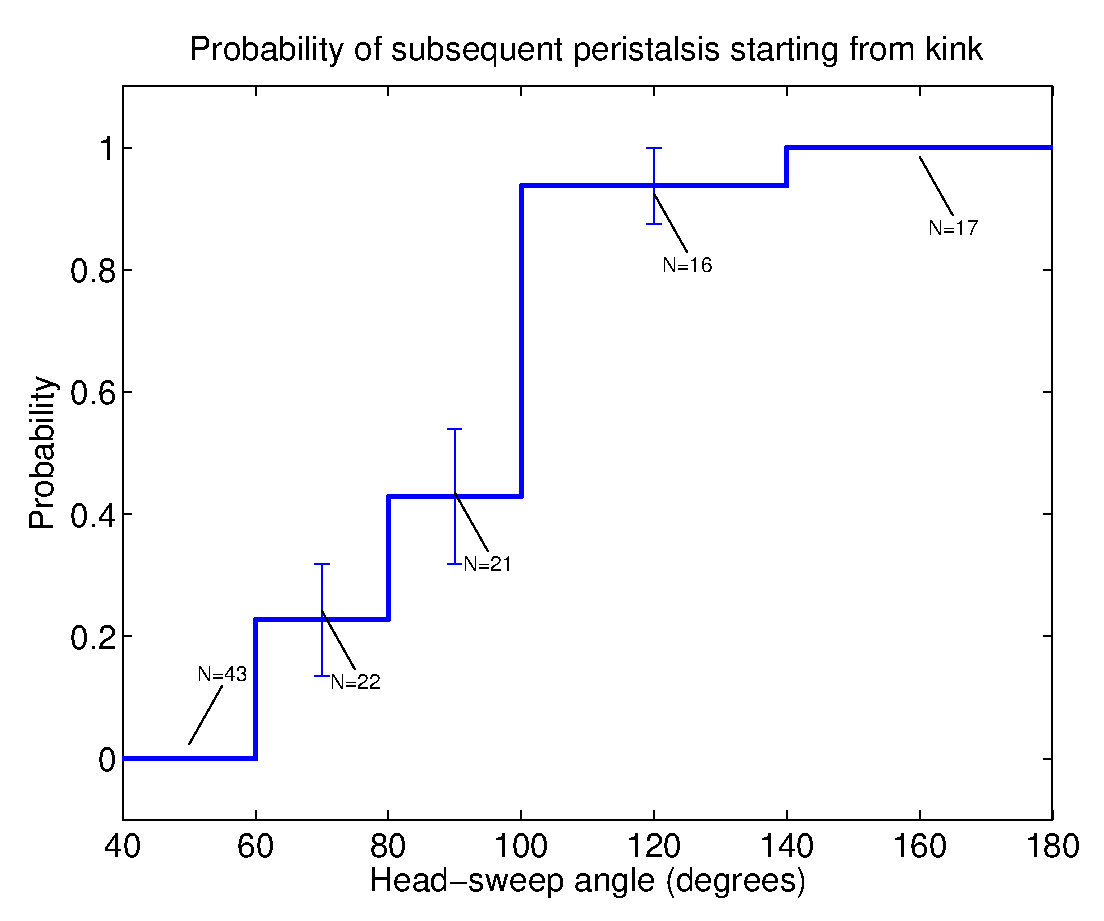
\includegraphics[height=5cm]{Figs/ProbKink.eps}
 \end{center}

 \begin{itemize}
 \item Transition is around $90-100\degs$.
 \item Varies from animal to animal.
 \item Not fully determined by angle.
 \end{itemize}
%
\end{frame}

%-------------Slide--------------------------------------------------------

\begin{frame}{Possible explanations}
%
 \begin{itemize}
   \item Mechanical reason?

   $>90\degs$ tail would move wrong way.

   $<90\degs$ starting from kink would be slower.
   \vp

   \item Neural circuit?

   Stretch-sensors involved in locomotion pattern. If one side is already contracted, segment just anterior to kink might think peristaltic pulse has already reached it
   \vp

   \item Central pattern generator?

   Body re-coupling in mid-cycle -- dependence on \hs\ size?
 \end{itemize}
%
\end{frame}

%-------------Section--------------------------------------------------------

\section{Conclusions and future directions}

%%-------------Slide--------------------------------------------------------
%
%\begin{frame}{Double \hs}
%%
% Large ($104^\circ$) rejected followed by small ($65^\circ$) accepted.
%
% %
% \begin{center}
%   \movie[width=150px,height=150px,showcontrols=true,loop,poster]{}
%   {double_hs.avi}
% \end{center}
% %
%%
%\end{frame}
%
%%-------------Slide--------------------------------------------------------
%
%\begin{frame}{Backwards Peristalsis}
%%
% %
% \begin{center}
%   \movie[width=180px,height=180px,showcontrols=true,loop,poster]{}
%   {back_prop.avi}
% \end{center}
% %
%%
%\end{frame}
%
%
%-------------Slide--------------------------------------------------------

\begin{frame}{Conclusions}
%
 All \hs s start at the same segments. Same circuits? Decision on size of \hs\ made later?
 \note[item]{need to interfere with sensory input during \hs\ optogenetically.}

 \vp Navigation results from combining two basic motor programs: peristalsis and asymmetric contraction. Pathway from sensory input $\to$ motor output simpler than previously thought.
 \note[item]{only need to decide when to switch programs}

 \vp No ``unbending'' motor program. \note[item]{can only reject by going other way.}

 \vp Large \hs s: subsequent peristalsis starts at kink. Shows that peristalsis can start anywhere. Implications for circuits that control forward motion.
 \note[item]{peristalsis initiator not localised}

%
\end{frame}


%-------------Slide--------------------------------------------------------

\begin{frame}{Future directions}
%
 Interfere with motor patterns (optogenetically).\note[item]{requires next point}

 \vp Fully automate image analysis. \note[item]{machine learning - training data}

 \vp Other stimuli.
 \note[item]{we did temperature, could do odour. light difficult. Unlikely to be any difference.}

 \vp Reverse crawling, hunching, and rolling.\note[item]{nociceptive and rapid avoidance responses}
%
\end{frame}



%
%% Press Ctrl-D to insert a new slide
%
%
%-------------Slide--------------------------------------------------------

\begin{frame}{Acknowledgements}
%
 Thanks to:
 \begin{itemize}
   \item Konlin Shen
   \item Anji Tang
   \item Mason Klein
   \item Liz Kane
   \item Ashley Carter
   \item Aravi Samuel
   \item Garrity lab
 \end{itemize}
 \note[item]{Last slide!}
%
\end{frame}

%-------------Slide--------------------------------------------------------

\begin{frame}[allowframebreaks]{References}
%

 {\small
 \bibliographystyle{unsrt_slides}
 \bibliography{larva}
 }
%
\end{frame}

%-------------Slide--------------------------------------------------------

\begin{frame}[label=fr_toothpaste]{Toothpasting}
%
 %
 \begin{center}
   %\hypertarget{fr:toothpaste}{
   \movie[width=180px,height=180px,showcontrols=true,loop]
   {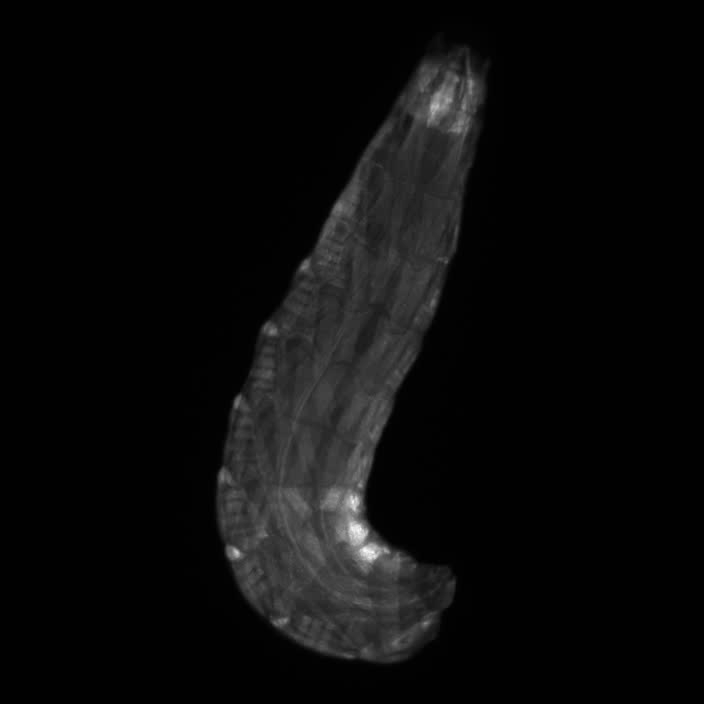
\includegraphics[width=180px,height=180px]{Firstframe/toothpaste.png}}
   {Vids/toothpaste.avi}
   %}
 \end{center}
 %
 \hyperlink{fr_loco}{\beamerbutton{back}}
%
\end{frame}

%-----End----------------------------------------------------------------

\end{document}
